\documentclass[border=2pt,tikz]{standalone}
\usepackage{tikz}
\usepackage{amsmath}
\usepackage{amssymb}

\begin{document}

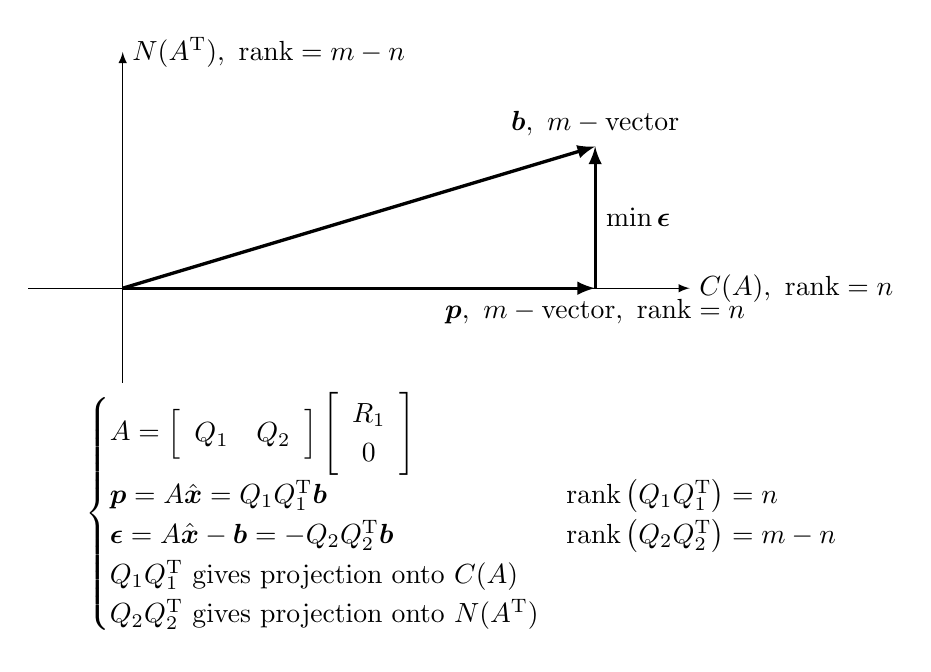
\begin{tikzpicture}[scale=6]

\draw[->,>=latex] (-0.2, 0.0) -- (1.2, 0.0) node [right] {$C(A),\ \mathrm{rank}=n$} ;
\draw[->,>=latex] ( 0.0,-0.2) -- (0.0, 0.5) node [right] {$N(A^{\mathrm T}),\ \mathrm{rank}=m-n$} ;

\draw[very thick, ->,>=latex] (0.0, 0.0) -- (1.0, 0.3) node [above] {$\boldsymbol{b},\ m-\text{vector}$} ;
\draw[very thick, ->,>=latex] (1.0, 0.0) -- node [right] {$\min \boldsymbol{\epsilon}$} (1.0, 0.3) ;
\draw[very thick, ->,>=latex] (0.0, 0.0) -- (1.0, 0.0) node [below] {$\boldsymbol{p},\ m-\text{vector},\ \mathrm{rank}=n$} ;

\node[below right] at (-0.1,-0.2) {$\begin{cases}
A=\left[\begin{array}{cc}
Q_{1} & Q_{2}\end{array}\right]\left[\begin{array}{c}
R_{1}\\
0
\end{array}\right]\\
\boldsymbol{p}=A\hat{\boldsymbol{x}}=Q_{1}Q_{1}^{\mathrm{T}}\boldsymbol{b} & \mathrm{rank}\left(Q_{1}Q_{1}^{\mathrm{T}}\right)=n\\
\boldsymbol{\epsilon}=A\hat{\boldsymbol{x}}-\boldsymbol{b}=-Q_{2}Q_{2}^{\mathrm{T}}\boldsymbol{b} & \mathrm{rank}\left(Q_{2}Q_{2}^{\mathrm{T}}\right)=m-n\\
Q_{1}Q_{1}^{\mathrm{T}}\text{ gives projection onto }C(A)\\
Q_{2}Q_{2}^{\mathrm{T}}\text{ gives projection onto }N(A^{\mathrm{T}})
\end{cases}$} ;

\end{tikzpicture}

\end{document}

